\chapter{UML DIAGRAMS}

\section{Introduction}
Unified Modeling Language (UML) diagrams are used to represent the design and structure of the system in a visual form. These diagrams help in understanding how different components of the system interact with each other. In this project, UML diagrams are used to explain the functionality, structure, and workflow.

\section{Use Case Diagram (Figure 6.1)}
The use case diagram represents the interaction between the user and the system. In this project, the main actor is the administrator, who interacts with the system through a web interface. 
\begin{figure}[H]
\centering
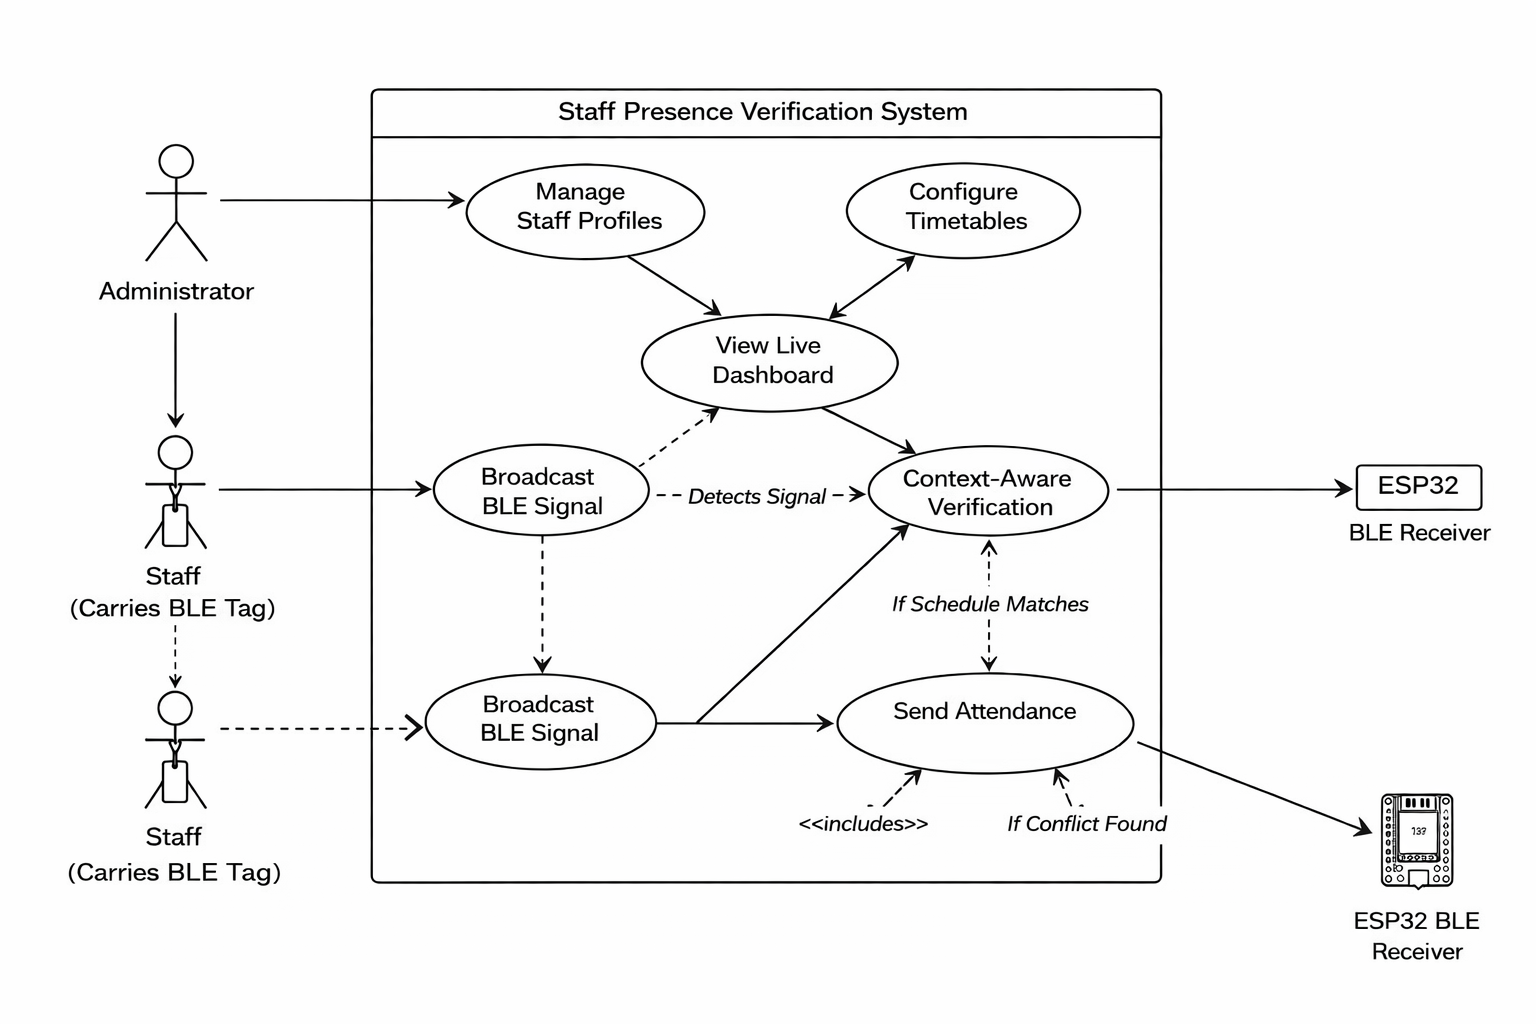
\includegraphics[width=0.6\textwidth]{images/use_case_diagram.png}
\caption{Use Case Diagram}
\end{figure}
The administrator performs operations such as registering staff details, assigning BLE tags, managing timetable information, and monitoring attendance records. The system automatically detects staff presence using BLE signals and updates attendance data accordingly.

\section{Class Diagram (Figure 6.2)}
The class diagram represents the structure of the system by showing different classes and their relationships. 
\begin{figure}[H]
\centering
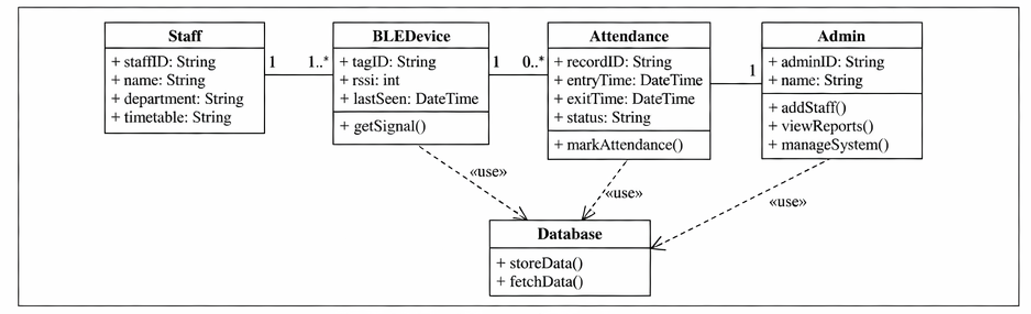
\includegraphics[width=0.8\textwidth]{images/class_diagram.png}
\caption{Class Diagram}
\end{figure}
In this project, the system is divided into several classes such as Staff, BLEDevice, Attendance, Admin, and Database. The Staff class contains attributes like staff ID, name, department, and timetable. The BLEDevice class stores information about the BLE tag and signal data. The Attendance class manages attendance records including entry time, exit time, and status.

\section{Sequence Diagram (Figure 6.3)}
The sequence diagram shows the step-by-step interaction between different components of the system over time. 
\begin{figure}[H]
\centering
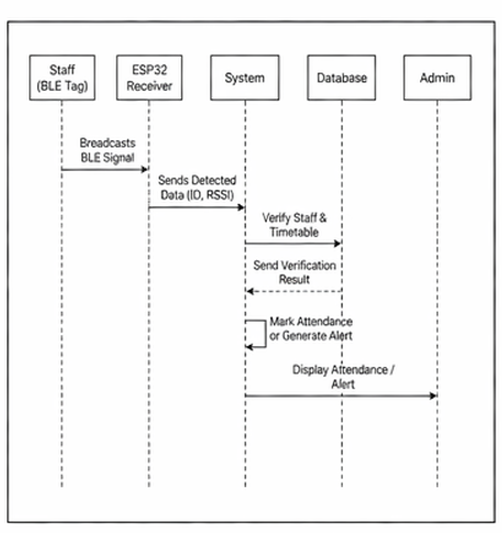
\includegraphics[width=0.8\textwidth]{images/sequence_diagram.png}
\caption{Sequence Diagram}
\end{figure}
In this project, the sequence begins when a staff member enters the classroom with a BLE ID card. The ESP32 receiver detects the BLE signal and sends the data to the system. The system processes the data and verifies it with the stored database.

\section{Activity Diagram (Figure 6.4)}
The activity diagram represents the workflow of the system from start to end. 
\begin{figure}[H]
\centering
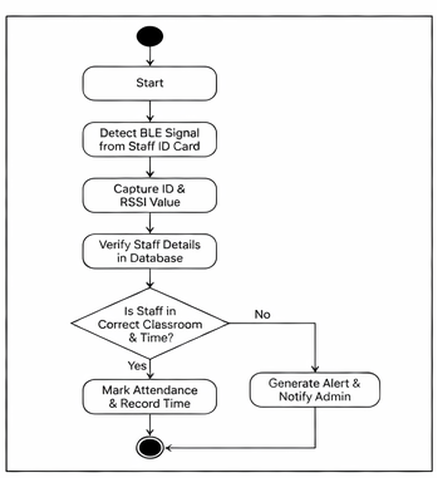
\includegraphics[width=0.6\textwidth]{images/activity_diagram.png}
\caption{Activity Diagram}
\end{figure}
The process starts with the detection of BLE signals by the ESP32 receiver. The system then processes the signal and extracts the unique ID. If the staff member is present in the correct location at the correct time, attendance is marked.
